\documentclass[10pt,twoside, fleqn]{memoir}
\usepackage{graphicx}
\usepackage{hyperref} % HYPERLINKS
\usepackage[nomain,acronym,toc]{glossaries}
\makeglossaries
\usepackage{xcolor}
\hypersetup{
    colorlinks,
    linkcolor={blue!50!black},
    citecolor={blue!50!black},
    urlcolor={blue!80!black}
}
\definecolor{warningbackground}{RGB}{252,226,158}
\definecolor{infobackground}{RGB}{217,237,247}
\definecolor{infoforeground}{RGB}{58,135,173}
\definecolor{infoborder}{RGB}{188,232,241}
\usepackage{environ}
\usepackage{tikz}
\usetikzlibrary{fit,backgrounds,calc}

%\usepackage[T1]{fontenc}
%\usepackage{mathpazo} % USE PALATINO FONT
%\usepackage[latin1]{inputenc}
%\usepackage[xindy]{imakeidx}

%\usepackage[british]{babel}
%\usepackage[framed, numbered, autolinebreaks]{mcode}
%\usepackage{listings}

%

%\usepackage[font=footnotesize]{caption}
%\usepackage{subcaption}
%\usepackage{pdflscape} %Landscape pages
%\usepackage{pdfpages}
%\usepackage{amsmath}
%\usepackage{amssymb}
%\usepackage{gensymb} %Degree sign
%\usepackage{footnote} %Footnotes in tabulars
%\usepackage{xcolor,framed,marginnote,blindtext}
%\colorlet{shadecolor}{blue!10}
%
%
%\usepackage{tikz} %TO CREATE BLOCK DIAGRAMS
%%\usetikzlibrary{external}
%%\tikzexternalize
%%\tikzset{external/mode=graphics if exists}
%
%\usetikzlibrary{shapes,arrows}
%\usetikzlibrary{positioning}
%
%\setcounter{tocdepth}{2} % DEPTH OF TABLE OF CONTENTS; 2= SUBSECTIONS INCLUDED
%\setcounter{secnumdepth}{2} % SUBSECTIONS ARE NUMBERED
%
%\usetikzlibrary{positioning}



%% BEGIN TITLE

\makeatletter
\def\maketitle{%
  \null
  \thispagestyle{empty}%
  \vfill
  \begin{center}\leavevmode
    \normalfont
    {\LARGE\raggedleft \@author\par}%
    \hrulefill\par
    {\huge\raggedright \@title\par}%
    \vskip 1cm
%    {\Large \@date\par}%
  \end{center}%
  \vfill
  \null
  \cleardoublepage
  }
\makeatother
\author{RYMAPT}
\title{Ethoscope user manual and documentation}
\date{23 February 2015}


\newacronym{ddye}{D$_{\text{dye}}$}{donor dye, ex. Alexa 488}
\newacronym[description={\glslink{r0}{F\"{o}rster distance}}]{R0}{$R_{0}$}{F\"{o}rster distance}
\newglossaryentry{r0}{name=\glslink{R0}{\ensuremath{R_{0}}},text=F\"{o}rster distance,description={F\"{o}rster distance, where 50\% ...}, sort=R}
\newglossaryentry{kdeac}{name=\glslink{R0}{\ensuremath{k_{DEAC}}},text=$k_{DEAC}$, description={is the rate of deactivation from ... and emission)}, sort=k}

% A
\newacronym{af}{AF}{Auto Focus}
\newacronym{apt}{APT}{Advanced Positioning Technology}

% C
\newacronym{ccd}{CCD}{Charge Coupled Device}

% D
\newacronym{dio}{DIO}{Digital InputOutput}
\newacronym{dpss}{DPSS}{Diode Pump Solid State}

% F
\newacronym{fov}{FOV}{Field of View}

% G
\newacronym{gui}{GUI}{Graphic User Interface}

% I
\newacronym{ide}{IDE}{Integrated Development Environment}
\newacronym{ifd}{IFD}{Image File Directory}
\newacronym{ir}{IR}{Infra-red}

% L
\newacronym{led}{LED}{Light Emitting Diode}
\newacronym{lsm}{LSM}{Laser Sheet Microscopy}

% M
\newacronym{mosfet}{MOSFET}{Metal Oxyde Semiconductor Field-Effect Transistor }

% N
\newacronym{nas}{NAS}{Network Attached Storage}
\newacronym{ntc}{NTC}{Negative Temperature Coefficient}

% P
\newacronym{pcb}{PCB}{Printed Circuit Board}
\newacronym{pwm}{PWM}{Pulse Width Modulation}
\newacronym{psf}{PSF}{Point Spread Function}

% S
\newacronym{scl}{SCL}{Serial Clock Line}
\newacronym{sda}{SDA}{Serial DAta line}
\newacronym{shr}{SHR}{Synology Hybrid Raid}
\newacronym{svn}{SVN}{Apache SubVersion}

% T
\newacronym{tif}{TIFF}{Tagged Image File Format}
\newacronym{tps}{TPS}{Thinnest Part of the Sheet}

% U
\newacronym{usb}{USB}{Universal Serial Bus}

% R
\newacronym{roi}{ROI}{Region Of Interest} 


%%% BEGIN DOCUMENT
\makeindex
\begin{document}

\let\cleardoublepage\clearpage


\maketitle
\frontmatter

\null\vfill
\begin{center}
\begin{figure}
  \centering
  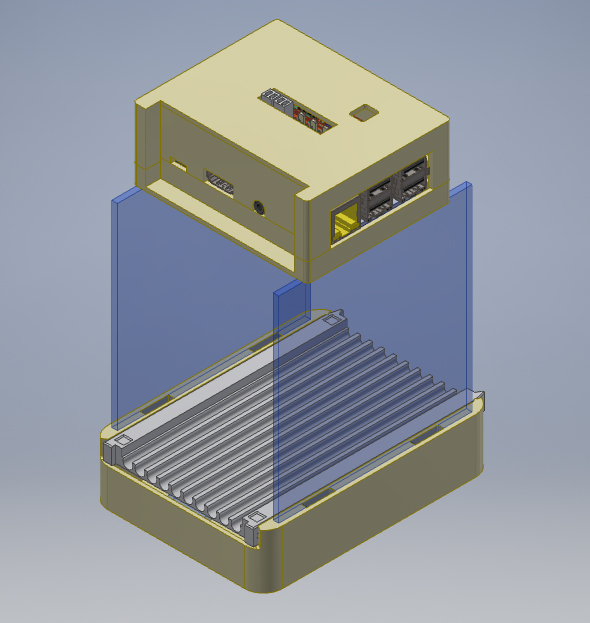
\includegraphics[width=0.80\textwidth]{./images/isometric.jpg}
  \label{fig:Intro}
\end{figure}
\end{center}
\begin{flushleft}
\textit{Ethoscope user manual and documentation}\newline
\newline
RYMAPT - 2017\newline info@rymapt.com
\bigskip

\end{flushleft}
\let\cleardoublepage\clearpage

\newpage
\tableofcontents

\mainmatter
\sloppy

\newenvironment{SpecialPar}
  {\begin{shaded}\marginnote{\fbox{NOTE}}}
  {\end{shaded}}

%%%%%%%%%%%%%%%%%%%%%%%
% COMMAND TO CREATE A WARNING BOX
\NewEnviron{alertinfo}[1]
{
    \begin{tikzpicture}
    \node[inner sep=0pt,
          draw=infoborder,
          line width=1.2pt,
          fill=infobackground] (box) {\parbox[t]{.99\textwidth}
        {%
            \begin{minipage}{.15\textwidth}
                \centering\tikz[scale=3]
                \node[scale=1]
                {
                    
\includegraphics[scale=0.04]{./images/warning.png}
                };
            \end{minipage}%
           \begin{minipage}{.80\textwidth}
                \vskip 10pt
                \textbf{\textcolor{infoforeground}{#1}}\par\smallskip
                \textcolor{infoforeground}{\BODY}
                \par\smallskip
            \end{minipage}\hfill
        }%
    };

    \end{tikzpicture}
}
%%%%%%%%%%%%%%%%%%%%%%%


%%% INCLUDE CHAPTERS
%\include{ch_Introduction}
\chapter{Hardware description}\label{ch:hardware}
The Ethoscope is comprised of the following parts:
\begin{description}
  \item[Top unit] This contains the main components of the Ethoscope, such as the processing unit, the camera and the environmental shield (optional). The components are enclosed in a plastic shell.
  \item[Base unit] The unit acts as a base for the whole Ethoscope and as a support and alignment tool for the arena. The base unit also contains the strip of \gls{led} used to provide \gls{ir} illumination to the arena.
  \item[Arena] The arena defines the experiment to be performed. The basic arena, provided with the standard kit, provides support for up to twenty glass tubes, each one defined as a \gls{roi}. Three black dots in the corner of the arena are used by the software to determine a spatial system of reference.
  \item[Side walls] The walls connect the base to the top unit and ensure a correct distance between camera and arena. The standard walls are made of 3~mm acrylic sheet.
\end{description}

\section{Setup}\label{ch:setup}
 
\chapter{Software description}\label{ch:software}

\section{Network Setup}\label{sec:network}
To communicate with the Ethoscope devices, the control computer, smart phone or tablet (henceforth ``client'')
must be on the same network as the Ethoscopes. Each ethoscope unit comes pre-configured to join the WiFi network
of the supplied router. The client can connect to this network using the WiFi details printed on the case of
the router, or by connecting an ethernet cable from the client to the router.

The control interface for each Ethoscope is available at the address printed on the case (e.g.
\textit{http://ethoscope-01234.local} where \textit{01234} is a hexadecimal number unique to each unit). If this
address does not work see section \ref{sec:ipaddress}. On connecting to this address, you will be presented with
a list of all Ethoscope devices on the network. Note that it is possible to control all Ethoscopes on the network
by connecting to any one individual Ethoscope.

\section{Connecting with an IP address}\label{sec:ipaddress}
Ethoscope control is through a web interface, which in principle should work with any javascript enabled browser.
However one needs to know the address to connect on. Ethoscope devices advertise their presence using the mDNS
(also called ZeroConf, or Bonjour on Apple devices or Avahi on Linux devices) and LLMNR protocols using the
hostname printed on the ethoscope case.

Some clients, notably Android, are not able to resolve mDNS or LLMNR addresses and this address will not work.
In these cases it is necessary to connect using the device's IP address. The IP address can be found either
by logging on to the router and looking at the list of connected devices, or by using third party apps that
scan the network and list all mDNS capable devices.

For Android there is \textbf{ZeroConf Browser}\footnote{https://play.google.com/store/apps/details?id=com.melloware.zeroconf}
and for iOS there is \textbf{Flame Services Browser}\footnote{https://itunes.apple.com/gb/app/flame/id325206381}.
Note that these apps are unaffiliated with Rymapt and we cannot offer support on their use. They are however quite
simple, just open the app and select the ethoscope device, the IP address will be shown underneath and will look
similar to \textit{192.168.0.102}. Type that address into your browser and you will be presented with the Ethoscope
control interface.

%% Need to add decent instructions for logging on to the router, but I don't have one with me so I'll add
%% less vague instructions later
To access the router's interface and see a list of connected devices, connect to \textit{http://192.168.0.1} and
use the username ``admin'' and password ``admin''. Go to the DHCP page and all devices on the network will be
listed.

\section{Advanced use}\label{sec:advanced}
\subsection{MySQL access}\label{subsec:mysql}
The recorded data can be retrieved from each ethoscope by accessing the MySQL database running on
the device. There are many open source and proprietry tools that can access MySQL databases. Read
only access is available with the username ``ethoscope'' and password ``ethoscope'' on the normal MySQL
port (3306).
 
\subsection{SSH access}\label{subsec:mysql}
It is possible to logon to each ethoscope directly to perform custom configuration, however this is
discouraged because careless use can render the devices inoperable. In some cases this can invalidate
your warranty. For normal use it should never be necessary to access the device directly.

Advanced users who know what they're doing can access the device on the normal SSH port (22) with
the username ``pi'' and the password printed on the case of the ethoscope.

\subsection{Using a different network}\label{subsec:mysql}
Ethoscope units will work on another network with no configuration if connected by an ethernet cable.
WiFi configuration is not possible with the current release of the software but will come in a
future update. It is however possible to SSH on to the device and configure other WiFi networks by
hand using the ``wpa\textunderscore{}cli'' Linux tool, but this is for advanced users only.

Please note that using Ethoscopes on open networks is discouraged since there is no encryption or
security in the current software release. Anybody on the same network can read all data and
start/stop runs. Rymapt is working to remedy this, and encrypted connections with access control
will be available in a future update along with guided WiFi setup.

%\include{ch_MainGUI}
%\include{ch_Calibration}
%\include{ch_Tracking}
%\include{ch_PSF}

%%% APPENDIX
%\include{ch_Appendix}


%%% GLOSSARY
%\printglossaries
%\printglossary[type=\acronymtype]
\printglossary[type=\acronymtype,title=Abbreviations]

%%% BIBLIOGRAPHY
%\bibliographystyle{unsrt}
%\bibliography{./../Bibliography/myBibliography}


\end{document} 